\documentclass[10pt]{article}

\usepackage{parskip}
\usepackage[margin=1in]{geometry} 
\usepackage{tikz}
\usetikzlibrary{positioning}
\usepackage{amsmath,amsthm,amssymb, graphicx, multicol, array}
\usepackage{enumitem}
\usepackage{amssymb}
\usepackage{float}
\usepackage{href-ul}
 
\newcommand{\N}{\mathbb{N}}
\newcommand{\Z}{\mathbb{Z}}
 
\newenvironment{problem}[2][Problem]{\begin{trivlist}
\item[\hskip \labelsep {\bfseries #1}\hskip \labelsep {\bfseries #2.}]}{\end{trivlist}}

\begin{document}
 
\title{Foundations of causal inference (cont.)\\Experimental Designs}
\author{Jakob Sverre Alexandersen\\
GRA4158 Marketing and the Analysis of Experiments and Quasi-Experiments\\
Lecture 5}
\maketitle

\tableofcontents
\newpage
\section{Online ad experiments in marketing and their problems}
\textbf{Recall}
\begin{itemize}
    \item \textbf{Intent to treat (ITT)}
    \begin{itemize}
        \item Under non-compliance, where $D(T) $ does not always equal $T $
        \item ITT is a valid estimate of the effect of the assignment $T $, but \underline{not} the effect of treatment $D $
    \end{itemize}
    \item \textbf{Local average treatment effect (LATE)}
    \begin{itemize}
        \item Average treatment effect of the compliers
    \end{itemize}
    \item $\text{ITT} = \text{ITT}_D\times\text{LATE} = p(\text{complier})\times\text{LATE}$
\end{itemize}
\subsection{Relation between ITT and ATET/ATE}
\begin{itemize}
    \item ITT is often seen as a conservative estimate of ATE / ATET 
    \begin{itemize}
        \item ITT is typically smaller than LATE under monotonicity (no defiers)
        \item $\text{ITT} = \text{ITT}_D\times\text{LATE} $
        \item $\text{ITT}_D = \mathbb{E}[D_i = 1 | T_i = 1] - \mathbb{E}[D_i = 1 | T_i = 0] $ is between 0 and 1 $\to $ share of compliers
    \end{itemize}
    \item However, this relation is only valid when both the instrument (here, assignment $T $) and the focal treatment variable (here, exposure $D $) are binary: $T, D\in\{0, 1\} $
    \begin{itemize}
        \item Otherwise, $\mathbb{E}[D_i = 1 | T_i = 1] - \mathbb{E}[D_i = 1 | T_i = 0] $ also does not need to be in the 0 to 1 range
        \item We will look at that situation again when discussing instrumental variables in more detail 
    \end{itemize}
\end{itemize}
\subsection{When is LATE = ATET?}
\begin{itemize}
    \item One-sided non-compliance in the treatment group 
    \begin{itemize}
        \item When the treatment is only available to the treatment group, the compliers are exactly the same group as the treatment population (ATET)
        \item We only have compliers and never-takers, or $D_i(T_i) = 1 $ only for $T_i = 1 $
    \end{itemize}
    \item Perfect compliance 
    \begin{itemize}
        \item If every individual complies with their assignment, i.e., $p(\text{complier}) = 100\% $ or $D_i(T_i) = T_i $
    \end{itemize}
    \item Homogenous effects 
    \begin{itemize}
        \item If the effect of compliers and always-takers are the same, then LATE = ATET
        \item If the effect of compliers and all others are the same, then LATE = ATE 
        \begin{itemize}
            \item i.e., there is \textbf{no treatment effect heterogeneity}
        \end{itemize}
    \end{itemize}
\end{itemize}
\textbf{A typical question in (digital) marketing}
\begin{itemize}
    \item Is it worth spending money on (digital) advertising?
    \item Is there an incremental effect on (digital) advertising?
    \begin{itemize}
        \item What would have happened if the advertising was not present?
        \item The difference in the outcome in the absence and presence of the focal advertisement (treatment)
    \end{itemize}
    \item Again, advertising exposure is not random. People are explicitly targeted for advertising where they show interest in products 
    \begin{itemize}
        \item We need a randomized experiment (or full information about all targeting variables $\to $ usually impossible)
    \end{itemize}
    \item Many ad platforms offer tools for ad experiments; i.e., randomized A/B tests
\end{itemize}

\subsection{Single-ad study vs. multi-ad studies and causal inference / divergent delivery}
\subsubsection{The problem with divergent delivery}
\begin{itemize}
    \item In online experiments, there is often a difference between users assigned to an experimental group adn those that are actually exposed to the ad 
    \begin{itemize}
        \item Non-compliance
    \end{itemize}
    \item Randomization is based on the user-level 
    \begin{itemize}
        \item All users who are eligible to see the ad 
    \end{itemize}
    \item But not all users in the treatment group will be exposed to the ad 
    \begin{itemize}
        \item Exposure is decided on an incidence-level (each time an ad is loaded)
    \end{itemize}
    \item The targeting and real-time auctioning process exposes users to the ads depending on their consumer profile, a prediction of whether they are likely to respond, and competitors' bissing behavior 
    \begin{itemize}
        \item Consequently, the exposed users are not a random sample of eligible users 
        \begin{itemize}
            \item Divergent delivery // non-random compliance
        \end{itemize}
    \end{itemize}
\end{itemize}
\subsubsection{Two main types of online ad experiments --- divergent delivery}
\textbf{Single-ad study with holdout/control}
\begin{itemize}
    \item Typical question: is there an incremental effect of the ad on an outcome of interest?
    \item Consumers are randomly divided into treatment group and a holdout/control group 
    \item Consumers in the treatment group are eligible to see the ad, but not all consumers will see the ad 
    \item Consumers in the control group will not see the ad 
    \begin{itemize}
        \item One-sided compliance, we are able to calculate LATE or even ATET in some situations 
    \end{itemize}
\end{itemize}
\textbf{Multiuple-ad study without holdout}
\begin{itemize}
    \item Typical question: Which of the two versions of an ad is better?
    \item Classic A/B testing: Consumers are randomly assigned to group A or B
    \item Consumers in group A will only see ad A
    \item Not all consumers will see the ad because of targeting (exposure is not random, only assignment)
    \begin{itemize}
        \item We are not able to make inferences about incremental effects of A over B; i.e., about causal effects
    \end{itemize}
\end{itemize}
\newpage 
\subsection{Interpretation of A/B test (multiple-ad study) with targeting}
\begin{itemize}
    \item Under divergent delivery, results may be interpreted as the combined effect of ad content and platform's targeting 
    \begin{itemize}
        \item Whether this matters to the experimenter depends on the goal of the experiment 
    \end{itemize}
    \item You cannot say that ad A is better than ad B (in general or for the specified audience)
    \item You can only say that ad A is better on this platform given the specific targeting algorithm and campaign settings
    \item Ad B might be similar or better than A on a different platform, with a different algorithm, with different optimization objective
\end{itemize}
\subsection{When is divergent validity a problem for multi-ad studies?}
\begin{figure}[H]
    \centering
    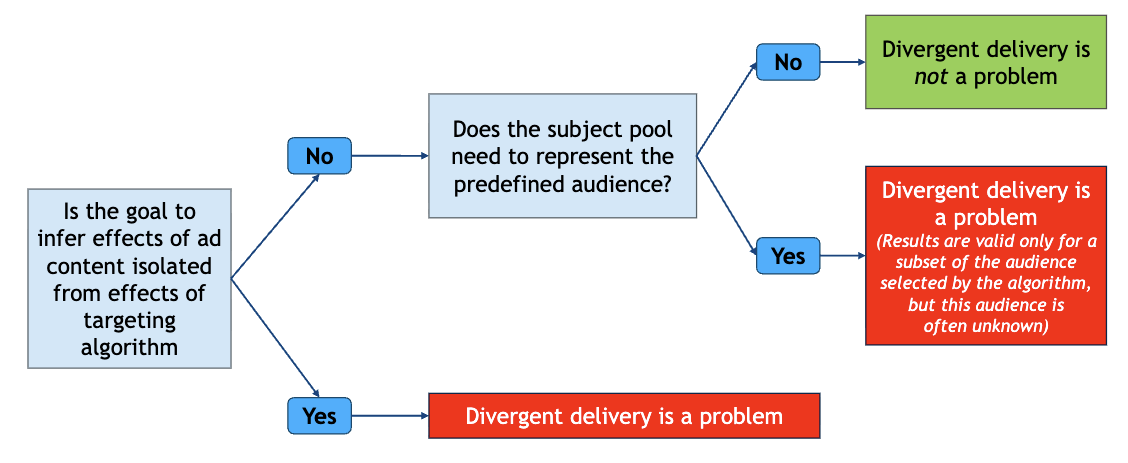
\includegraphics[width=0.8\textwidth]{image.png}
\end{figure}
\subsection{Single-ad study with holdout/control}
\begin{itemize}
    \item Typically, we have one-sides non-compliance (users in the control group do not see the ads)
    \item We may be able to estimate ITT and LATE, but typically they will not be a good estimate of ATE or ATET, because compliance is not random and there may be treatment effect heterogeneity
\end{itemize}
\subsection{Identification of outcomes}
\begin{itemize}
    \item How to track individual outcomes (e.g., website visits, registrations, purchases) in the non-treatment group (i.e., those users that will not see the ad is often challenging)
    \begin{itemize}
        \item The tracking cookie is ususally placed with the ad 
        \item We need a platform that identifies control user outcomes 
        \item We may need to be able to differentiate between control users that would have been exposed 
    \end{itemize}
    \item Not all marketing relevant metrics can be used as outcomes 
    \begin{itemize}
        \item All metrics that require seeing an ad are not possible (e.g., click-through rate: CTR)
    \end{itemize}
\end{itemize}
\newpage 
\subsection{The ideal situation --- ATET}
\begin{itemize}
    \item Ad effectiveness as the difference between customers who saw the ad and consumers who would have seen the ad, had they not been in the control group
\end{itemize}
\begin{figure}[H]
    \centering
    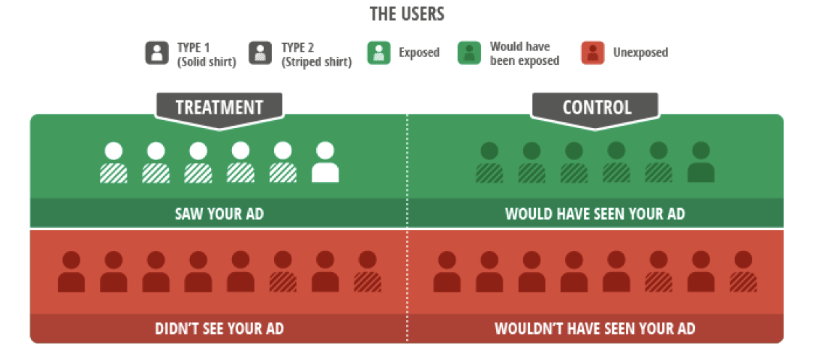
\includegraphics[width=0.8\textwidth]{image2.png}
\end{figure}

\subsection{Conclusions}
\begin{itemize}
    \item Significant selection effects usually lead to overestimating the ad effect 
    \item Observational methods are usually not able to estimate the ad effect well enough 
    \begin{itemize}
        \item Even with excessive control variables they overestimate in most of the studies 
        \item No single observational method is systematically better
    \end{itemize}
    \item Randomized experiments (AB testing) is the gold standard to avoid selection effects 
    \item Individuals usually vary in their strength of the treatment effect 
    \begin{itemize}
        \item Instead of looking only at averages we can also try to explore heterogeneity in the treatment effects $\to $ estimate a CATE 
        \begin{itemize}
            \item e.g., group specific estimates, interaction effects
        \end{itemize}
    \end{itemize}
    \item Individuals might not always comply with treatment assignment
    \begin{itemize}
        \item One-sided or two-sided non-compliance
        \item Compliers, always-takers, never-takers, defiers 
        \item Treatment effect estimators: ITT, ATET, and LATE 
    \end{itemize}
    \item For measuring (online) advertising effectiveness we need properly designed experiments 
    \begin{itemize}
        \item We need understanding about one-sided non-compliance etc. 
        \item Even excessive amounts of control variables are not able to properly control for all selection effects
    \end{itemize}
\end{itemize}
\newpage 
\subsection{A bit on binary outcomes and causal inference}
\begin{itemize}
    \item In marketing, we often have binary outcomes (choices, events, etc.)
    \begin{itemize}
        \item Responded (yes/no), purchased (yes/no), choice (A/B)
        \item Marketers are often interested in conversion rates
    \end{itemize}
\end{itemize}

\begin{center}
    \begin{tabular}{|c|c|c|c|}
        \hline 
        \textbf{Group} & \textbf{Purchased (1)} & \textbf{Did not purchase (0)} & \textbf{Total}\\\hline 
        \textbf{Ad} & 18 & 82 & 100\\\hline 
        \textbf{No ad} & 10 & 90 & 100\\\hline 
    \end{tabular}
\end{center}
\begin{itemize}
    \item Three (four) different focal measures
    \begin{itemize}
        \item Risk difference 
        \item Risk ratio (or lift)
        \item Odds ratio
    \end{itemize}
    \item \textbf{Risk difference}:
    \begin{itemize}
        \item 18\% - 10\% = 8\% $\to $ our ATE
        \item The ad increases the probability of purchasing by 8 pct 
    \end{itemize}
    \item \textbf{Risk ratio:}
    \begin{itemize}
        \item Compares the probability of an event happening in one group vs. another
        \item $\frac{18}{10} = 1.8\% $
        \item People taking seeing the ad are 1.8 times as likely to purchase compared to those not seeing ads 
    \end{itemize}
    \item \textbf{Odds ratio:}
    \begin{itemize}
        \item Compares the odds of an event, not the probability; i.e., the ratio of successes to failures
        \item Odds in treatment: $\frac{18}{82}\approx 0.22 $
        \item Odds in control: $\frac{10}{90}\approx 0.11 \to \text{ odds ratio: }1.98$ (odds in treatment over odds in control)
        \item The odds of purchasing are 2.68 times higher when seeing the ad vs not seeing the ad 
    \end{itemize}
    \item In marketing A/B testing, lift is often used as a relative measure of improvement in a rate (conversion, click-through, retention)
    \item The risk-ratio (RR) is almost the same as ``lift'', just expressed as a ratio rather than a percent: 
    \begin{gather*}
        \text{RR} = \frac{\mathbb{E}[Y = 1 | T = 1]}{\mathbb{E}[Y = 1 | T = 0]}\\
        \\
        \text{Lift} = \frac{\mathbb{E}[Y = 1 | T = 1] - \mathbb{E}[Y = 1 | T = 0]}{\mathbb{E}[Y = 1 | T = 0]} = 1 - \text{RR} = \frac{\text{Risk difference}}{\mathbb{E}[Y = 1 | T = 0]} = \frac{\text{ATE}}{\text{Baseline conversion}}
    \end{gather*}
\end{itemize}
\textbf{Previous example}
\begin{itemize}
    \item Lift = $\frac{0.18 - 0.1}{0.1} = 1 - 1.8 = 80\% $
    \item Ads improve conversion rate by $80\% $
\end{itemize}
\newpage 
\subsection{Logistic regression}
\begin{itemize}
    \item Using logistic regression seems natural when having binary outcomes 
    \item However, 
    \begin{itemize}
        \item Logistic regression is typically not estimating ATE (the risk difference) nor the risk ratio (lift) which is what decision-makers are typically interested in 
        \item It estimates the treatment effect on the odds-ratio (often not what decision-makers are interested in)
    \end{itemize}
    \item Logistic regression is superior to linear probability models (linear regression on binary outcomes) when it comes to predictions, but not necessarily causal inference (\textit{depending on the type of question})
\end{itemize}
\section{Experimental Design}
\subsection{Why it matters}
\begin{itemize}
    \item Experimental design is the planning stage of an experiment 
    \item The task of the experiment is to get an answer to a business/research problem 
    \begin{itemize}
        \item The task of experiment design is getting the right data so you can get an answer that's valid 
    \end{itemize}
    \item From: what is it that we want to study? ... via... how do we implement the experiment in a way that it creates valid conclusions to our questions? ... to... analyzing the data in a way that reflects the experimental design / actual implementation
    \begin{itemize}
        \item Usually, the planning makes more than 80\% of the time and resources, while less than 20\% is data analysis 
    \end{itemize}
    \item Without careful planning of your experiment, you are wasting resources because even the cleverest data might not recover the core question 
    \begin{itemize}
        \item Ensuring that statistical tests / data analyses are able to answer the question we want to solve 
    \end{itemize}
\end{itemize}
\subsection{Within vs. between subject experiments}
\begin{itemize}
    \item \textbf{Between subjects}
    \begin{itemize}
        \item Treatment and control measure are taken from \textbf{different experimental groups} with different test subjects 
        \item Together with \textbf{random assignment} it is most effective in isolating the treatment effect
    \end{itemize}
    \item \textbf{Within subjects}
    \begin{itemize}
        \item Treatment and control measure are taken from the same test subjects at \textbf{different points in time}
        \item Need to assure that \textbf{nothing changes} between the two time points beside the treatment 
        \item Prone to several biases 
        \begin{itemize}
            \item Demand effects 
            \item Order and carryover effects 
            \item Changes in the environment 
        \end{itemize}
    \end{itemize}
\end{itemize}
\newpage 
\subsection{Manipulating the independent variable}
\begin{itemize}
    \item A core challenge in the design of every experiment is to find the right way of \textbf{varying the treatment} (i.e., the \textbf{independent variable})
    \begin{itemize}
        \item Selecting the right treatment and control condition(s)
    \end{itemize}
    \item What is the \textbf{counterfactual?}
    \begin{itemize}
        \item Is it the absence of something?
        \item Or is it an explicit alternative?
        \item What is the focal concept that we want to test / research?
        \item How can we correctly implement the alternatives without inference?
    \end{itemize}
    \item Balance between realism and a clear definition of the desired manipulation
    \begin{itemize}
        \item Internal vs. external validity
    \end{itemize}
    \item Variation of the independent variable must meet two important requirements: 
    \begin{itemize}
        \item Effectiveness: The treatment must be effective in the sense that the focal concept is indeed varied 
        \item Control: The treatment must guarantee that any spects other than the focal independent variable are not unintentionally varied 
    \end{itemize}
\end{itemize}
\subsection{Examples}
\begin{itemize}
    \item \textbf{Scarcity queues in E-commerce}
    \begin{itemize}
        \item Causal question: does displaying a scarcity queue (few products left in stock) influence purchase intentions / sales in e-commerce stores?
    \end{itemize}
    \item \textbf{IV}: scarcity
    \begin{itemize}
        \item Treatment: displaying in-stock information 
        \item Counterfactual / control: ???
    \end{itemize}
    \item \textbf{Effectiveness}: is displaying in-stock information actually varying scarcity perception?
    \begin{itemize}
        \item Is the displayed number large/small enough to affect scarcity in a meaningful way?
        \item Manipulation check: measure scarcity?
    \end{itemize}
    \item \textbf{Control}: is displaying in-stock information varying any other variables than scarcity?
    \begin{itemize}
        \item e.g., it could signal popularity, etc. 
    \end{itemize}
\end{itemize}
\subsubsection{Compound treatment --- example}
\begin{itemize}
    \item You want to investigate the causal effect of a price discount on purchase decisions
    \item You run a typical A/B test
    \begin{itemize}
        \item You randomly assign customers to two groups 
        \item Customers in the treatment group get an email with the price discount 
        \item Customers in the control group do not get an email 
    \end{itemize}
    \item \textbf{Is the difference between the groups the effect of the price discount?}
    \begin{itemize}
        \item I'd say no --- the effect is most likely from spamming customers with emails. To get the true effect we must simply do a price change on the website with no other actions 
    \end{itemize}
\end{itemize}
\newpage 
\subsubsection{Similar: Placebo effects}
\begin{itemize}
    \item You want to test the effect of receiving a medicine on reduction of pain 
    \item You run a typical A/B test 
    \begin{itemize}
        \item You randomly assign customers to two groups 
        \item People in the treatment group get the pill
        \item People in the control group do not get the pill
    \end{itemize}
    \item \textbf{Is the difference between groups the effect of the medicine?}
    \begin{itemize}
        \item No, because observed differences between the treatment and control group may be due to \textit{receiving the pill} and not because the medicine actually works
        \begin{itemize}
            \item Solution: also give a placebo pill to the control group 
        \end{itemize}
    \end{itemize}
\end{itemize}
\subsection{Measuring the dependent variable(s)}
\begin{itemize}
    \item Another core challenge is to find a good way to measure the dependent variable(s); i.e., the intended outcome variable(s)
    \item What is the variable that we are interested in?
    \begin{itemize}
        \item Are we able to measure it directly? Do we need proxy variables to measure it indirectly?
        \item Are we able to measure it in all treatment (and control) conditions the same way?
        \begin{itemize}
            \item Is measuremetn possible in the absence of treatment?
        \end{itemize}
    \end{itemize}
    \item Does the type of measure introduce threats to validity?
    \begin{itemize}
        \item e.g., demand effects, anchoring and carry-over effects, social desirability, etc.?
    \end{itemize}
    \item Do we need to capture additional variables to understand the process and mechanism of the treatment better (i.e., mediators)?
\end{itemize}
\subsection{Validity of experiments}
\begin{itemize}
    \item \textbf{Internal validity}
    \begin{itemize}
        \item Refers to whether the treatment of actually caused the observed effects o the dependent variable(s)
        \item Can we actually estimate the treatment effect within the given context and for our particular sample?
        \begin{itemize}
            \item Fails when there are differences between treatment groups (other than the treatment itself) that affect the outcome and that we cannot control 
            \item Directly associated with the design of the experiment
        \end{itemize}
    \end{itemize}
    \item \textbf{External validity}
    \begin{itemize}
        \item Refers to whether the cause-and-effect relationships found in the experiment can be generalized 
        \item Can we extrapolate our estimates to other settings / pupulations / time?
        \begin{itemize}
            \item Fails when the treatment effect is different
            \begin{itemize}
                \item outside the evaluation environment
                \item or for other groups of people 
            \end{itemize}
            \item How realistic / representative is the experiment for real environments in which the treatment should be applied?
        \end{itemize}
    \end{itemize}
\end{itemize}
\newpage 
\subsection{Internal validity}
\subsubsection{Some common threats to internal validity of experiments}
\begin{itemize}
    \item Statistical conclusion validity
    \item The experimental protocol
    \begin{itemize}
        \item Potential outcomes not independent of assignment: presence of selection effects 
        \item Non-compliance
        \item Interference / violation of SUTVA 
        \item (Differntial) attrition 
        \item Time effects 
    \end{itemize}
    \item Awareness about the experiment
    \begin{itemize}
        \item Hawthorne effect 
        \item Demand effects 
    \end{itemize}
    \item The measurement of the outcome 
    \begin{itemize}
        \item Differential measures 
        \item Ambiguous temporal precedence 
    \end{itemize}
\end{itemize}
\subsubsection{Threats to internal validity --- statistical conclusion validity}
\begin{itemize}
    \item Are the statistical assumptions of the method in use fulfilled?
    \begin{itemize}
        \item Affects our ability to accurately estimate the treatment effect and correct inference from data 
        \item Some potential problems: 
        \begin{itemize}
            \item Misspecification of the functional term (e.g., linear, non-linear)
            \item Misspecification of DV: continuous vs. discrete 
            \item Misspecification of the error structure: e.g., heteroskedasicity or autocorrelated error terms 
            \item Ignoring measurement error 
        \end{itemize}
    \end{itemize}
    \item Knowledge of the design is important to choose the right statistical framework for estimating the causal effects under given circumstances 
    \begin{itemize}
        \item Different designs require different statistical methods 
        \item Some designs may never allow correct statistical inference 
    \end{itemize}
\end{itemize}
\newpage 
\subsubsection{Threats to internal validity --- The experimental protocol}
\begin{itemize}
    \item Failure of randomzation / selection effects 
    \begin{itemize}
        \item If the assignment mechanism is not random, we cannot rule out selection effects 
        \item We can test on observed pre-treatment variables for equivalence of groups 
        \item Or we need to require conditional independence (i.e., after controlling for observables we achieve independence)
    \end{itemize}
    \item Non-compliance
    \begin{itemize}
        \item Subjects do not comply with their treatment status 
        \item e.g., compliers, always-takers, never-takers, defiers
    \end{itemize}
    \item Violation of SUTVA (stable unit treatment value assumption)
    \begin{itemize}
        \item Interference: potential outcomes are not independent of the treatment status of other individuals 
    \end{itemize}
\end{itemize}
\subsection{Stratified random assignment}
\begin{itemize}
    \item Does not randomize on the population level, but within more homogenous subgroups
    \begin{itemize}
        \item Assigns loyalty card members with 50\% probability to treatment and control 
    \end{itemize}
    \item Endures better balance for each of the characteristics on which we build subgroups/strata
    \begin{itemize}
        \item Characteristics should be potentially confounders where balancing is important 
    \end{itemize}
    \item Important if the characteristics have low prevalence in the population or we have small sample sizes
    \begin{itemize}
        \item Example: we have a sample of 100 customers of an airline out of which 2 are heavy frequent flyers. We split the 100 customers into two randomly assigned groups. What is the probability that the frequent flyers end up in one group?
    \end{itemize}
    \item Important if we want to use this characteristic to analyze heterogeneous treatment effects 
    \begin{itemize}
        \item e.g., sub-group specific ATEs 
    \end{itemize}
\end{itemize}
\subsection{Interference problems in marketing --- examples}
\begin{itemize}
    \item \textbf{Word-of-mouth}
    \begin{itemize}
        \item Treated individuals may affect the outcomes for untreated individuals by talking about the treatment 
    \end{itemize}
    \item \textbf{Observation}
    \begin{itemize}
        \item Untreated individuals may observe purchasing behavior of treated individuals and adapt their purchase behavior
    \end{itemize}
    \item \textbf{Crossover}
    \begin{itemize}
        \item Individuals who are assigned to the control are (accidentally) also exposed to the treatment 
    \end{itemize}
    \item \textbf{Network effects}
    \begin{itemize}
        \item Whether other individuals in the network are treated or untreated increases/decreases the consumption utility (i.e., changes the potential outcomes)
    \end{itemize}
    \item Treatment effects are not independent of the treatment status of other individuals 
\end{itemize}
\newpage 
\subsection{Threats to internal validity --- the experimental protocol}
\textbf{Differential attrition}
\begin{itemize}
    \item Attrition: Participants leave the experiment before all measurements are completed 
    \item Differential attrition: Drop out in the treatment group is larger or smaller than in the control group due to reasons of the experiment / drop out is not independent of the potential outcomes 
    \begin{itemize}
        \item e.g., treatment or no treatment causes some people to drop out 
    \end{itemize}
\end{itemize}

\textbf{Time effects}
\begin{itemize}
    \item When treatments are administered at two different times, outside events, learning, or other changes in the environment can influence the treatment effect 
\end{itemize}
\subsection{Threats to internal validity --- awareness about the experiment}
\textbf{Hawthorne effect}
\begin{itemize}
    \item If individuals know that they are part of an experiment, they may change their behavior due to the attention and monitoring they receive 
\end{itemize}
\textbf{Demand effects}
\begin{itemize}
    \item Participants guess the purpose or goals if the experiment and try to conform (or disconform) with it 
    \item They change their behavior in favor for or against the hypothesis $\to $ increasing or decreasing the treatment effect 
\end{itemize}

Ideally people should be \textbf{unaware of the experiment} but consider ethical consquences 

\subsection{Threats to internal validity --- the measurement of the outcome}
\textbf{Differential measures}
\begin{itemize}
    \item Sometimes it is difficult to measure the same outcome (or with the same reliability) in the different treatment groups 
    \item Psychological measures may change meaning due to treatment (or absence thereof)
    \item Actual behavior might be harder to observe in the absence or presence of the treatment
    \begin{itemize}
        \item e.g., tracking cookies that come with an advertisement, but is not placed without the ad 
        \item e.g., engagement (e.g., clicks) is not possible if not seeing an ad 
    \end{itemize}
\end{itemize}

\textbf{Ambiguous temporal precedence}
\begin{itemize}
    \item The type of measurement does not allow to distinguish whether treatment actually lies before the outcome or after $\to $ resolution of the measurement is too broad (e.g., day, week, month)
\end{itemize}
\end{document}